For a given system, Pareto optimal states (of which there may be infinite) form a set in performance space.  A Pareto optimal state is said to be located within the region of trait space called the \textit{Pareto front}. In Fig. \ref{fig:paretoFront} this is illustrated for up to three dimensions using light blue to encode Pareto front regions. 

\begin{figure}[h]
\centering
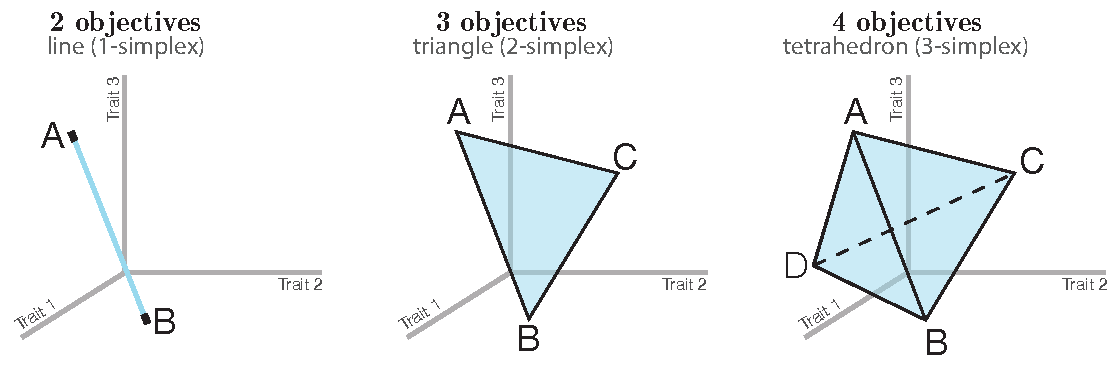
\includegraphics[width=\linewidth]{figures/paretoFronts.pdf} 
\caption{Pareto front regions (blue) for up to three tasks in trait-space. In the \textbf{2 tasks}-case the Pareto front spans the edge connecting tasks A and B. For \textbf{3 tasks} and \textbf{4 tasks} Pareto fronts are the area and volume, respectively, of the simplex spanned by the set of tasks.}
\label{fig:paretoFront}
\end{figure}
Recent findings in evolution research, based on the principle of pareto optimality, shows that such tradeoffs tend to drive biological systems toward configurations where trait, i.e. physical traits, are highly defined within ranges. Pareto optimal datapoints in any such system, assume the shape of a simplex when projected onto hyperplanes